% Copyright (c) 2018 Victorien Elvinger
% Code licensed under GPLv3 (https://www.gnu.org/licenses/gpl-3.0.en.html).
% Content licensed under CC-BY 4.0 (https://creativecommons.org/licenses/by/4.0/).

\documentclass[xcolor=table,t]{beamer}
% t: vertical flush of every frame (local override possible)

\usepackage[utf8]{inputenc}

% Theorem
\usepackage{amsthm}

% Math
\let\Bbbk\relax % redefined in newtxmath (imported by acmart)

\usepackage{amssymb}
\usepackage{mathtools} % fix amsmath bugs + better typeset

\newcommand*{\trm}[1]{\operatorname{\mathsf{#1}}} % custom math term

% Math - paired notations
% Each commands
% - has a * version that scales to the size of the content
%   e.g. set*{x}
% - an option to specify delimiter size
%   e.g. set[\Big]{x}
%   among: \big, \Big, \bigg, \Bigg

\DeclarePairedDelimiter{\card}{\lvert}{\rvert}

\DeclarePairedDelimiter{\tuple}{\langle}{\rangle}

\providecommand{\given{}}
\newcommand*{\setgivenpart}[1][]{%
    \nonscript\:#1\vert\allowbreak\nonscript\:\mathopen{}}
\DeclarePairedDelimiterX{\set}[1]{\{}{\}}{%
    \renewcommand\given{\setgivenpart[\delimsize]}#1}
\DeclarePairedDelimiterX{\setopen}[1]{\{}{.}{%
    \renewcommand\given{\setgivenpart[\delimsize]}#1}
\DeclarePairedDelimiterX{\setclose}[1]{.}{\}}{%
    \renewcommand\given{\setgivenpart[\delimsize]}#1}

\newcommand*{\where}{\mathrel{\mathbf{where}}} % where keyword
\newcommand*{\when}{\mathrel{\mathbf{if}}} % if keyword
\newcommand*{\otherwise}{\mathrel{\mathbf{else}}} % if keyword

\usepackage{centernot}

\newcommand*{\lappend}{\operatorname{++}}
\newcommand*{\sminus}{-} % set minus
\newcommand*{\qsep}{\ldotp} % separator between quantifier and predicate

\newcommand*{\powerset}[1]{\mathcal{P} (#1)}
\newcommand*{\powerfset}[1]{\mathcal{P}_{\mathsf{fin}} (#1)}
\newcommand*{\defeq}{\overset{\scriptstyle\mathrm{def}}{=}}
\newcommand*{\defiff}{\overset{\scriptstyle\mathrm{def}}{\iff}}
\newcommand*{\assign}{\operatorname{\vcentcolon=}}
\newcommand{\irange}[2]{#1 \mathinner{\ldotp\ldotp} #2}
\newcommand*{\pto}{\hookrightarrow}
%\newcommand*{\pto}{\mathrel{\ooalign{\hfil$\mapstochar\mkern5mu$\hfil\cr$\to$\cr}}}

% rel (partial) equivalence relation
\newcommand*{\releq}{\overset{\scriptstyle\mathsf{rel}}{\simeq}}
\newcommand*{\rel}{\overset{\scriptstyle\mathsf{rel}}{\sim}}
\newcommand*{\nrel}{\overset{\scriptstyle\mathsf{rel}}{\nsim}}

% tran (partial) equivalence relation
\newcommand*{\traneq}{\overset{\scriptstyle\mathsf{tran}}{\simeq}}
\newcommand*{\tran}{\overset{\scriptstyle\mathsf{tran}}{\sim}}
\newcommand*{\ntran}{\overset{\scriptstyle\mathsf{tran}}{\nsim}}

% program order disjoint union of total order
\newcommand*{\po}{\overset{\scriptstyle\mathsf{po}}{\longrightarrow}}
\newcommand*{\npo}{\centernot\po}

% peer (partial) equivalence relation
\newcommand*{\peereq}{\overset{\scriptstyle\mathsf{peer}}{\simeq}}
\newcommand*{\peer}{\overset{\scriptstyle\mathsf{peer}}{\sim}}
\newcommand*{\npeer}{\overset{\scriptstyle\mathsf{peer}}{\nsim}}

% returns-before strict partial order
\newcommand*{\rb}{\overset{\scriptstyle\mathsf{rb}}{\longrightarrow}}
\newcommand*{\nrb}{\centernot\rb}

% arbitration strict total order
\newcommand*{\ar}{\overset{\scriptstyle\mathsf{ar}}{\longrightarrow}}

% visibility acyclic relation
\newcommand*{\vis}{\overset{\scriptstyle\mathsf{vis}}{\longrightarrow}}
\newcommand*{\nvis}{\centernot\vis}
\newcommand*{\viseq}{\leq_{\scriptstyle\mathsf{vis}}}
\newcommand*{\nviseq}{\nleq_{\scriptstyle\mathsf{vis}}}

% immediate dependency relation
\newcommand*{\idr}{\downarrow}

\newcommand\restr[2]{\ensuremath{\left.#1\right|_{#2}}}

\usepackage[backend=biber,defernumbers=true,bibstyle=trad-plain,citestyle=authortitle,sorting=none,maxbibnames=1,maxcitenames=1,]{biblatex}

\addbibresource{ref.bib}


% Theme
% -----------
\usetheme[
    sectionpage=simple,
    numbering=fraction
]{metropolis}
\setbeamertemplate{title page}[default]
\setbeamercolor{palette primary}{bg=black!80}
\setbeamerfont{footnote}{size=\scriptsize}
\setbeamersize{text margin left=4.4ex, text margin right=4.4ex}

\usepackage[scale=1.5]{ccicons}

\newenvironment{compactitemize}{%
\settowidth{\leftmargini}{\usebeamertemplate{itemize item}}%
\addtolength{\leftmargini}{\labelsep}%
\begin{itemize}%
}{\end{itemize}}

\newenvironment{compactenumerate}{%
\settowidth{\leftmargini}{\usebeamertemplate{enumerate item}}%
\addtolength{\leftmargini}{\labelsep}%
\begin{enumerate}%
}{\end{enumerate}}

% Meta-data
% ---------

\author{Victorien Elvinger}
\title{Synql: A CRDT-based Approach for Replicated Relational Databases with Integrity Constraints}
\institute{%
    
\includegraphics[height=2em]{fig/logo-loria.pdf}\hspace{2em}%
    
\includegraphics[height=2em]{fig/logo-ul.pdf}\hspace{2em}%
    
\includegraphics[height=2em]{fig/logo-cnrs.pdf}\hspace{2em}%
    
\includegraphics[height=2em]{fig/logo-inria.pdf}\hspace{2em}%
}
\date{June 2024}

\begin{document}
\maketitle

\begin{frame}{Adding collaborative features to applications}
    \begin{minipage}[c][.55\textheight][t]{\textwidth}
        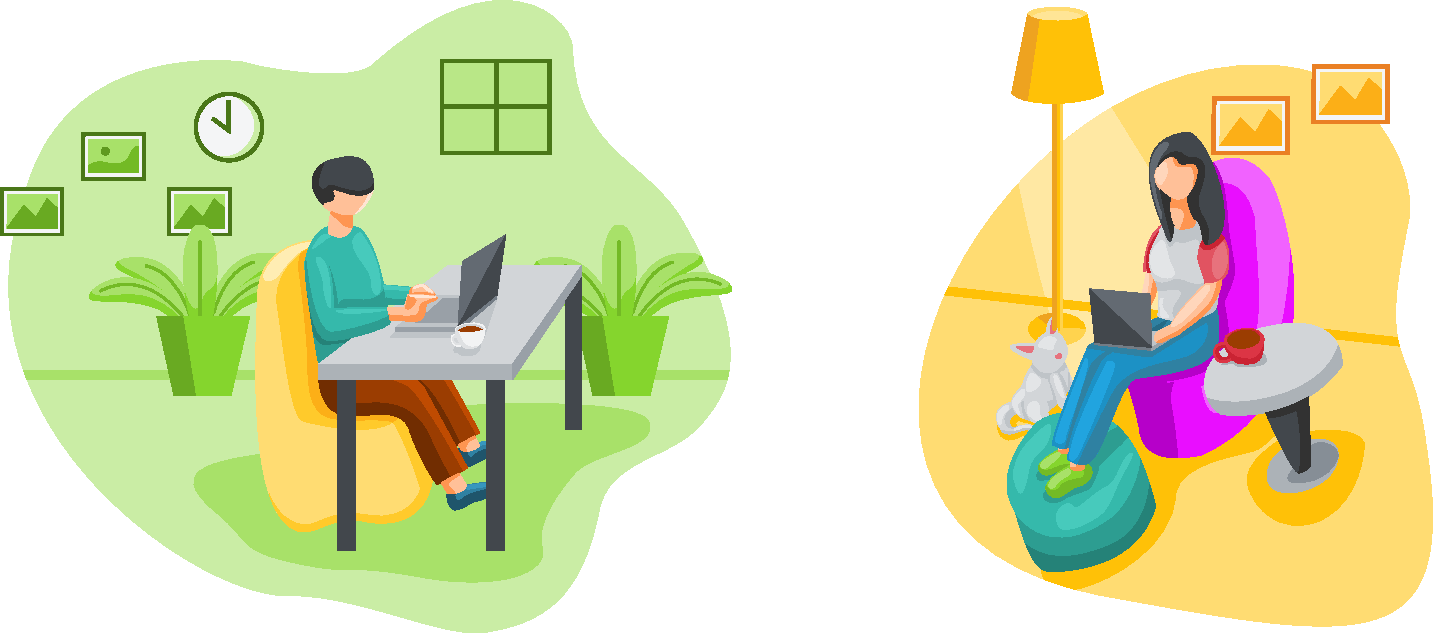
\includegraphics[width=0.9\textwidth]{fig/collab-activity.pdf}
    \end{minipage}
    \begin{minipage}{\textwidth}
        \begin{compactitemize}
            \item several persons \textbf{modify together} a shared content
            \begin{compactitemize}
                \item located at \textbf{different places}
                \item \textbf{simultaneous} modifications or at \textbf{distinct time}
            \end{compactitemize}
            \item adding collaborative features to applications is hard
            \begin{compactitemize}
                \item \textbf{sequential $\to$ concurrent} modifications
                \item \textbf{offline support}
            \end{compactitemize}
        \end{compactitemize}
    \end{minipage}
\end{frame}

\begin{frame}{Adding collaborative features to applications}
    \begin{minipage}[c][.55\textheight][t]{\textwidth}
        \centering
        \includegraphics<1>[width=.7\textwidth]{fig/app-sync.drawio.pdf}%
        \includegraphics<2>[width=.7\textwidth]{fig/app-data-sync.drawio.pdf}%
        \includegraphics<3>[width=.7\textwidth]{fig/app-db-sync.drawio.pdf}
    \end{minipage}
    \begin{minipage}{\textwidth}
        \begin{compactitemize}
            \item replicate the application?
            \begin{compactitemize}
                \item require dedicated development
            \end{compactitemize}
            \item<2-> \textbf{replicate the application data}\only<2->{\footcite{kleppmann2019localFirstSoft}}
            \item<3> SQLite is embedded in many applications
        \end{compactitemize}
    \end{minipage}
\end{frame}

\begin{frame}{Referential integrity}
    \begin{minipage}[c][.55\textheight][t]{\textwidth}
        \centering
        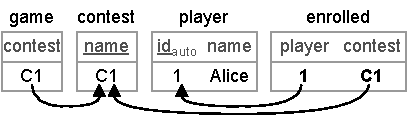
\includegraphics{fig/fk.drawio.pdf}
    \end{minipage}
    \begin{minipage}{\textwidth}
        \begin{compactitemize}
            \item ensure that the \textbf{target of a reference exists}
            \item the deletion of a target can result in
            \begin{compactitemize}
                \item the \textbf{abortion of the deletion}
                \item the \textbf{propagation of the deletion to its sources}
            \end{compactitemize}
        \end{compactitemize}
    \end{minipage}
\end{frame}

\begin{frame}{Referential integrity in face of concurrencies}
    \begin{minipage}[c][.55\textheight][t]{\textwidth}
        \centering
        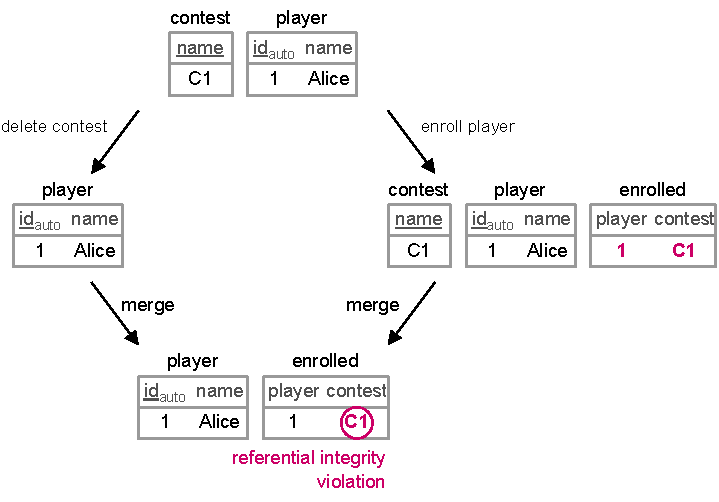
\includegraphics[height=.5\textheight]{fig/ref-violation.drawio.pdf}
    \end{minipage}
    \begin{minipage}{\textwidth}
        \begin{compactitemize}
            \item concurrent deletion and referencing of a row
        \end{compactitemize}
    \end{minipage}
\end{frame}

\begin{frame}{Replicating relational databases: already done?}
    \begin{minipage}[c][.55\textheight][t]{\textwidth}
        \centering
        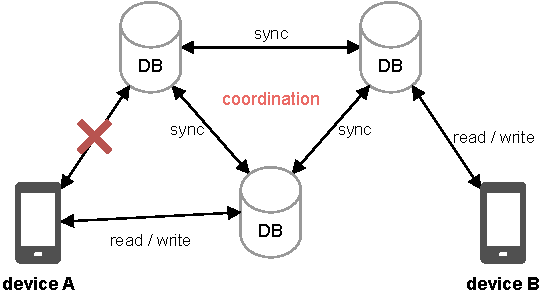
\includegraphics[height=.5\textheight]{fig/high-available-db.drawio.pdf}
    \end{minipage}
    \begin{minipage}{\textwidth}
        \begin{compactitemize}
            \item \textbf{client-server} architecture
            \item \textbf{coordination} to maintain \textbf{data integrity}\footcite{bailis2013HighlyAvailableTransactions}
        \end{compactitemize}
    \end{minipage}
\end{frame}

\begin{frame}{Coordination-less replication of relational databases}
    \begin{minipage}[c][.55\textheight][t]{\textwidth}
        \centering
        \includegraphics<1>[height=.5\textheight]{fig/gitlike-init.drawio.pdf}%
        \includegraphics<2>[height=.5\textheight]{fig/gitlike-clone.drawio.pdf}%
    \end{minipage}
    \begin{minipage}{\textwidth}
        \begin{compactitemize}
            \item Git-like \textbf{coordination-less} replication of relational databases\footcite{yu2020replicatedrelations}
            \begin{compactitemize}
                \item based on Conflict-free Replicated Data Types (CRDTs)
            \end{compactitemize}
            \item can \textbf{break data integrity and user intent}
            \item \textbf{not Strongly Convergent}
        \end{compactitemize}
        %\begin{compactenumerate}
        %    \item turn a database into a \textbf{replicated database}\footcite{yu2020replicatedrelations}
        %    \item<2> \textbf{clone} a replicated database
        %    \item<2> \textbf{synchronize} replicas
        %\end{compactenumerate}
    \end{minipage}
\end{frame}

\begin{frame}{Referential integrity maintenance - state of the art}
    \begin{minipage}[c][.55\textheight][t]{\textwidth}
        \centering
        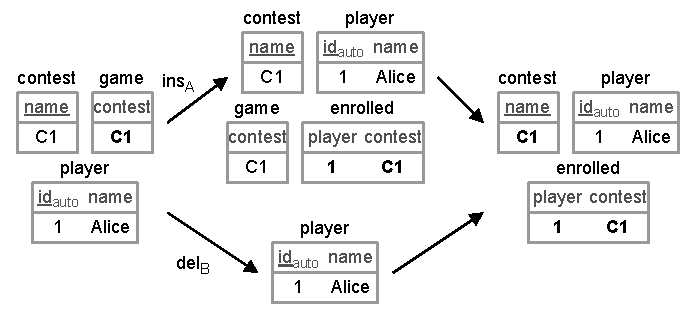
\includegraphics[height=.5\textheight]{fig/ref-ipa-issue.drawio.pdf}
    \end{minipage}
    \begin{minipage}{\textwidth}
        \begin{compactitemize}
            \item writes are compensated\footcite{balegas2018ipa} in order to ensure integrity
            \item the \emph{contest} is restored
            \item however, the \emph{game} is not restored
        \end{compactitemize}
    \end{minipage}
\end{frame}

\begin{frame}{Referential integrity maintenance - desired output}
    \begin{minipage}[c][.55\textheight][t]{\textwidth}
        \centering
        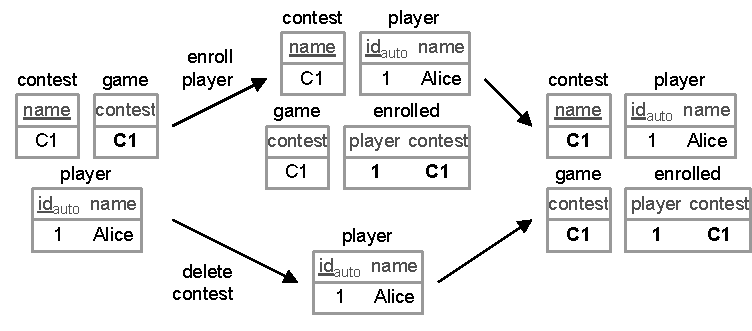
\includegraphics[height=.5\textheight]{fig/ref-synql.drawio.pdf}
    \end{minipage}
    \begin{minipage}{\textwidth}
        \begin{compactitemize}
            \item the \emph{game} should be restored
        \end{compactitemize}
    \end{minipage}
\end{frame}

\begin{frame}{Strong convergence}
    \begin{minipage}[c][.55\textheight][t]{\textwidth}
        \centering
        \vspace{4em}%
        \includegraphics<1>[height=.2\textheight]{fig/sec-sync.drawio.pdf}%
        \includegraphics<2>[height=.2\textheight]{fig/sec-convergent.drawio.pdf}
    \end{minipage}
    \begin{minipage}{\textwidth}
        \begin{compactitemize}
            \item property enforced by CRDTs\footcite{crdt2011shapiro}
            \item advantages:
            \begin{compactitemize}
                \item \textbf{low latency}
                \item \textbf{no flickering}
            \end{compactitemize}
        \end{compactitemize}
    \end{minipage}
\end{frame}

\begin{frame}[plain,standout]
    Can we replicate a relational database without any coordination that enforces Strong Convergence and maintains data integrity?
\end{frame}

\begin{frame}{Architecture overview}
    \begin{minipage}[c][.55\textheight][t]{\textwidth}
        \centering
        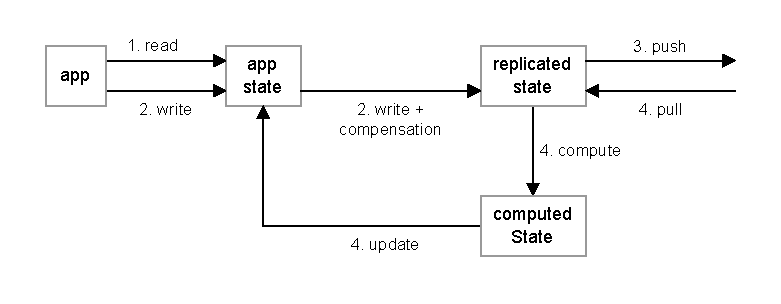
\includegraphics[height=.5\textheight]{fig/synql-overview.drawio.pdf}
    \end{minipage}
    \begin{minipage}{\textwidth}
        \begin{compactitemize}
            \item app read without overhead
            \item an app write triggers replicated state update
            \item push / pull in background
            \item a pull merges the received state and computes app state
        \end{compactitemize}
    \end{minipage}
\end{frame}

\begin{frame}{Replicated state: composing CRDTs}
    \begin{minipage}[c][.55\textheight][t]{\textwidth}
        \centering
        \includegraphics<1>[height=.5\textheight]{fig/repl-primitives.drawio.pdf}%
        \includegraphics<2>[height=.5\textheight]{fig/repl-primitives-flag.drawio.pdf}%
    \end{minipage}
    \begin{minipage}{\textwidth}
        \begin{compactitemize}
            \item \textbf{globally unique and monotonic timestamps}
            \begin{compactitemize}
                \item monotonic: greater than previously observed timestamps
            \end{compactitemize}
            \item Last-Writer-Win (LWW) Register\footcite{Johnson1975MaintenanceOfDuplicatedDatabase} \textbf{keeps the newest value}
            \item state of CLFlag computed from the \textbf{longest chain}
        \end{compactitemize}
    \end{minipage}
\end{frame}

\begin{frame}{Replicated state: composing CRDTs}
    \begin{minipage}[c][.55\textheight][t]{\textwidth}
        \centering
        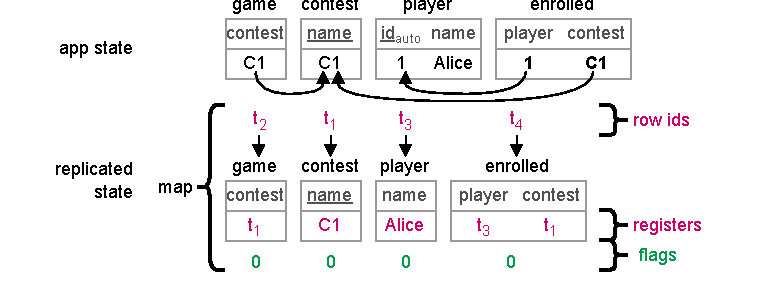
\includegraphics[height=.5\textheight]{fig/repl-state.drawio.pdf}
    \end{minipage}
    \begin{minipage}{\textwidth}
        \begin{compactitemize}
            \item \textbf{timestamps as row identifiers}
            \item a CL-Flag indicates if a row is removed
            \item a replicated attribute is a LWW-Register
            \item row identifiers as values of foreign keys
        \end{compactitemize}
    \end{minipage}
\end{frame}

\begin{frame}{Replicated state: composing CRDTs}
    \begin{minipage}[c][.55\textheight][t]{\textwidth}
        \centering
        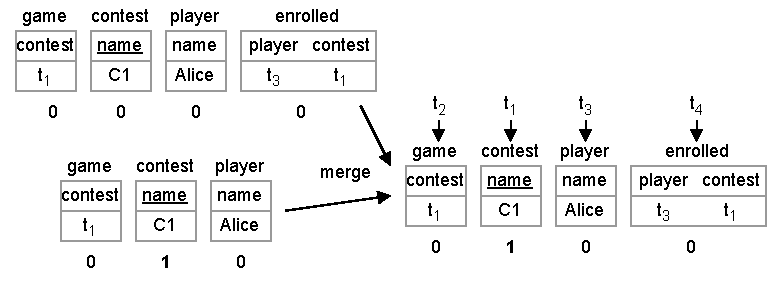
\includegraphics[height=.5\textheight]{fig/repl-state-merge.drawio.pdf}
    \end{minipage}
    \begin{minipage}{\textwidth}
        \begin{compactitemize}
            \item the replicated state encodes only the app write
        \end{compactitemize}
    \end{minipage}
\end{frame}

\begin{frame}{Compute app state from replicated state}
    \begin{minipage}[c][.55\textheight][t]{\textwidth}
        \centering
        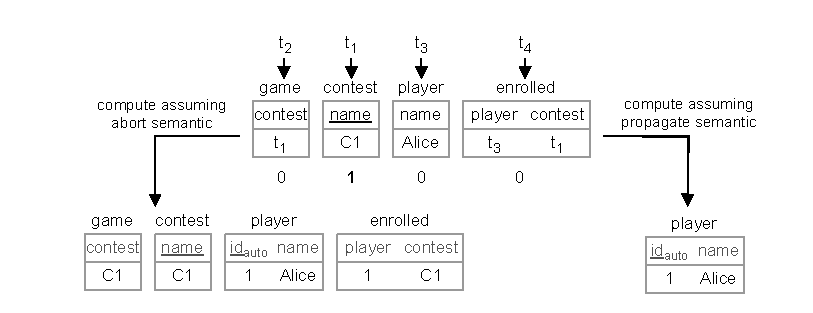
\includegraphics[height=.5\textheight]{fig/repl-state-compute.drawio.pdf}
    \end{minipage}
    \begin{minipage}{\textwidth}
        \begin{compactitemize}
            \item app state is \textbf{derived fom the replicated state}
            \item leverage database schema for selecting \textbf{computation semantic}
        \end{compactitemize}
    \end{minipage}
\end{frame}

\begin{frame}{Compensation of app writes}
    \begin{minipage}[c][.55\textheight][t]{\textwidth}
        \centering
        \includegraphics<1>[height=.5\textheight]{fig/repl-state-uncompensated.drawio.pdf}%
        \includegraphics<2>[height=.5\textheight]{fig/repl-state-compensated.drawio.pdf}%
    \end{minipage}
    \begin{minipage}{\textwidth}
        \begin{compactitemize}
            \item state computation can result in surprising effect on app writes
            \item<2> \textbf{app writes must be compensated} for ensuring user intent
        \end{compactitemize}
    \end{minipage}
\end{frame}

\begin{frame}{Conclusions}
    \begin{minipage}[c][.55\textheight][t]{\textwidth}
        \centering
        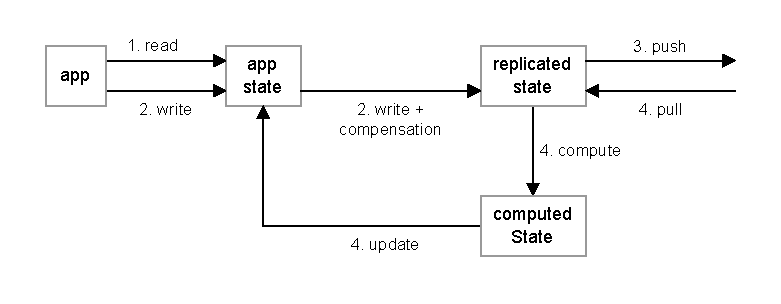
\includegraphics[height=.5\textheight]{fig/synql-overview.drawio.pdf}
    \end{minipage}
    \begin{minipage}{\textwidth}
        \begin{compactitemize}
            \item \textbf{coordination-less} replication of relational database
            \begin{compactitemize}
                \item \textbf{maintains data integrity}
                \item \textbf{Strongly Convergent}
            \end{compactitemize}
            \item composition of CRDTs + state computation + compensations
        \end{compactitemize}
    \end{minipage}
\end{frame}

\begin{frame}[plain]
    \begin{minipage}[c][.9\textheight][t]{\textwidth}
        \centering
        \vspace{0.2\textheight}
        
\includegraphics[height=.5\textheight]{fig/feedback.png}%
    \end{minipage}
    \begin{minipage}{\textwidth}
        \centering
        \ccby\hspace{3pt}4.0
    \end{minipage}
\end{frame}
\end{document}